\section{Traffic Volume}

In this section, users can search for the following traffic types:

\begin{itemize}
  \item Voice
  \item SMS
  \item Data
  \item ICX In/Out
  \item IGW In/Out
\end{itemize}

The common search area will include options to filter by these traffic types, and specific subsections will be added for each traffic category (Voice, SMS, Data, ICX In/Out, IGW In/Out).
\section{Traffic Volume - Subsection Common Search}

In this section, the user can filter traffic volume data by selecting the appropriate parameters from the following options:

\begin{itemize}
  \item \textbf{Traffic Type:} The user can select from the following options:
\end{itemize}

\begin{figure}[h]
  \begin{minipage}[b]{0.30\textwidth}
    \begin{itemize}
      \item Voice
      \item SMS
      \item Data
      \item ICX In/Out
      \item IGW In/Out
    \end{itemize}
  \end{minipage}
  \hfill
  \begin{minipage}[b]{0.45\textwidth}
    \centering
    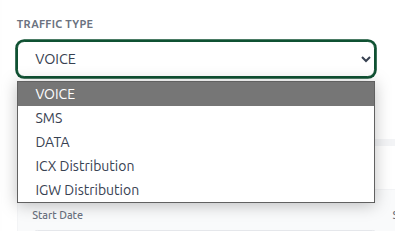
\includegraphics[width=\textwidth]{img/traffic/trafficTypes.png}  % Replace with the path to your image file
    \caption{Example of Traffic Type Selection}
  \end{minipage}
\end{figure}
\newpage
\begin{itemize}
  \item \textbf{Period:} The user can select a time period for data view, which can be one of the following:
\end{itemize}
\vspace{-50pt}
\begin{figure}[h]
  \begin{minipage}[b]{0.45\textwidth}

    \begin{itemize}
      \item Hourly
      \item Daily
      \item Monthly
      \item Yearly
    \end{itemize}
  \end{minipage}
  \hfill
  \begin{minipage}[b]{0.45\textwidth}
    \centering
    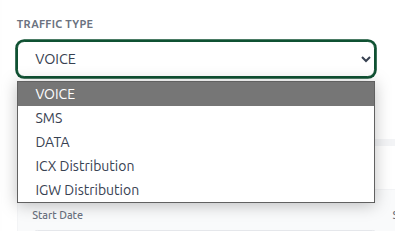
\includegraphics[width=\textwidth]{img/traffic/trafficTypes.png}  % Replace with the path to your image file
    \caption{Example of Period Selection}
  \end{minipage}
\end{figure}

\begin{itemize}
  \item \textbf{Quick Presets:} The user can quickly select a preset time range from the following options:
\end{itemize}

\begin{figure}[h]
  \begin{minipage}[b]{0.45\textwidth}
    \begin{itemize}
      \item Last Hour
      \item Last 24 Hours
      \item Last 7 Days
      \item Last 30 Days
      \item Last 90 Days
      \item Last Year
    \end{itemize}
  \end{minipage}
  \hfill
  \begin{minipage}[b]{0.45\textwidth}
    \centering
    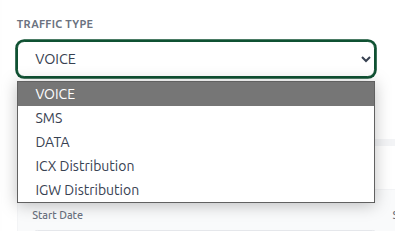
\includegraphics[width=\textwidth]{img/traffic/trafficTypes.png}  % Replace with the path to your image file
    \caption{Example of Quick Preset Selection}
  \end{minipage}
\end{figure}

\begin{itemize}
  \item \textbf{Start Date and Time:} The user selects the start date and, if the "Hourly" period is selected, the start time. The end date and end time are also configurable, but the start and end time are only active for the "Hourly" period.
\end{itemize}

\begin{itemize}
  \item \textbf{Operators:} The user can select operators as needed. The options include:
    \begin{itemize}
      \item All operators
      \item Single operator
      \item Multiple operators
    \end{itemize}
\end{itemize}

\begin{itemize}
  \item \textbf{Network Category:} The user can choose from various network categories, with all categories being selected by default.
\end{itemize}

\begin{itemize}
  \item \textbf{Direction:} The user can choose the direction for the traffic (inbound or outbound), with all directions being selected by default.
\end{itemize}

\begin{itemize}
  \item \textbf{Units:} The user can select between two unit types:
    \begin{itemize}
      \item Minute
      \item Count
    \end{itemize}
\end{itemize}

After applying the filters, the search results will update to reflect the selected parameters.

\clearpage
\begin{itemize}
  \item \textbf{Quick Presets:} The user can quickly select a preset time range from the following options:
\end{itemize}
\begin{figure}[h]
  \centering
  \begin{minipage}[b]{0.45\textwidth}  % Align with bottom to avoid the green space
    \begin{itemize}
      \item Last Hour
      \item Last 24 Hours
      \item Last 7 Days
      \item Last 30 Days
      \item Last 90 Days
      \item Last Year
    \end{itemize}
  \end{minipage}
  \hfill
  \begin{minipage}[t]{0.50\textwidth}  % Align with bottom to avoid the green space
    \centering
    \colorbox{gray!20}{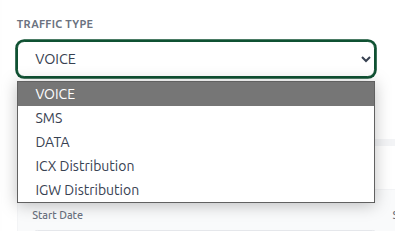
\includegraphics[width=1\linewidth]{img/traffic/trafficTypes.png}}
    \caption{Example of Quick Preset Selection}
  \end{minipage}
\end{figure}